\subsubsection{Glück} \label{glueck-1}



\todo[inline]{Verantwortlich: Minas}



Das Wort ``Glück'' wird im deutschsprachigen Gebrauch mit zwei unterschiedlichen Grundbedeutungen verwendet. 
In anderen Sprachen wird dieser Begriff auseinandergehalten z.B. im englischen als ``luck'' und ``happiness'' und im französichen als ``la bonne chance'' und ``le bonbeur''.
Im deutschen Sprachgebrauch muss zwischen den Glückszufall und die Glücksgabe, welches nicht erzwungen werden kann und zwischen das Glücklichsein, die Glückserfahrung und das Glückserlebnis unterschieden werden\cite{bien19}. \\

In diesem Szenario war es die Absicht anhand Fotos mit Texten und Musik im Hintergrund eine Glückserfahrung oder auch ein Glückserlebnis bei den Probanden auszulösen.
Abbildung \ref{fig-glueck} zeigt die hierfür verwendeten Bilder und deren Texte. \\

\begin{figure}[H] \centering
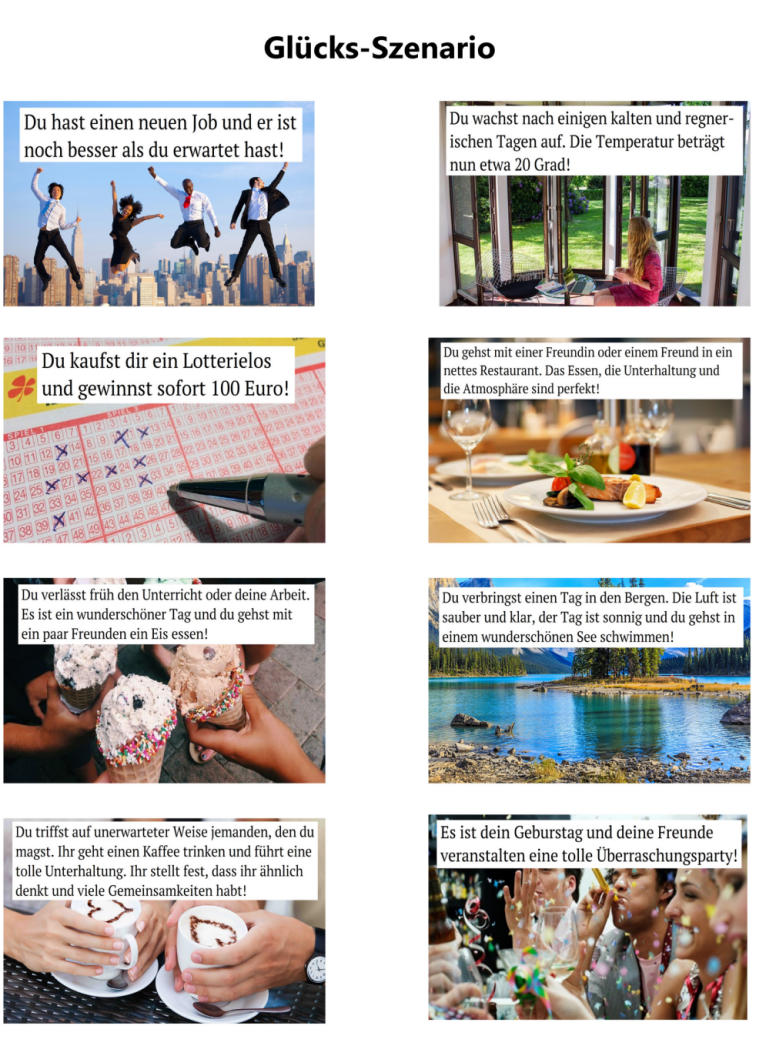
\includegraphics[width=12cm]{Images/gluck.png} 
\vspace{-0.3cm} 
\caption{Vignetten für das Glücks-Szenario.}
\label{fig-glueck} 
\end{figure}

Die Bilder wurden in einer PowerPoint-Präsentation abgespielt. 
Diese wechselten alle 30 Sekunden, während die Audiodatei im Hintergrund ablief.
Die Idee stammt von der wissenschaftlichen Publikation ``Mood inductions for four specific moods: A procedure employing guided imagery vignettes with music,'' von J. D. Mayer, J. P. Allen, und K. Beauregard. 
In dieser Publikation wurde versucht anhand Vignetten und Hintergrundmusik Glücksemotionen auszulösen.
Die verwendete Audiodatei aus der Publikation, welches aus dem Ballettstück ``Coppélia ou La Fille aux yeux d'émail'' stammte, wurde in diesem Szenario übernommen. 
Die aus der Publikation verwendeten Vignetten wurden insofern modifiziert, das einzelne durch eigene Vignetten ersetzt wurden.

